
\section{Latent Semantic Allocation}
\label{sec:lsa}

Topic model provides insights like
\begin{itemize}
	\item Can analyze topics. \eg, a certain topic includes specific words more than other topics. 
	\item A certain document's topic distribution (simplex)
\end{itemize}


pLSA: Latent Variable Model
$$P_{LSA}(w|d) = \sum_{z}P(w|z;\theta)P(z|d;\pi)$$
\begin{itemize}
	\item $w$: word
	\item $d$: document
	\item $z$: latent variable
\end{itemize}

Equivalently, 
$$P_{LSA}(d,w) = \sum_{z}P(w|z)P(d|z)p(z) = p(d)\sum_{z}P(w|z)P(z|d)$$

The probability of observing $n(w_i, d_j)$ occurrences of word $w_i$ in document $d_j$ is given by
$$p(w_i, d_j)^{n(w_i, d_j)}$$

The probability of observing the complete document collection is then given by the product of probabilities of observing every single word in every document with corresponding number of occurrences.

Then, the likelihood function becomes

$$L = \prod_{i=1}^{m}\prod_{j=1}^{n}p(w_i, d_j)^n(w_i, d_j)$$

The log-likelihood is then
\begin{align*}
	\mathcal{L} &= \sum_{i=1}^{m}\sum_{j=1}^{n}n(w_i, d_j)\log (p(w_i, d_j))\\
				&= \sum_{l=1}^kp(w_i|z_l)p(d_j|z_l)p(z_l) 
\end{align*}

Parameter Inference:
\begin{itemize}
	\item We cannot maximize the likelihood analytically because of the logarithm of the sum
	\item A standard procedure is to use \textit{EM}. 
\end{itemize}




\section{Latent Dirichlet Allocation}
\label{sec:topic_modeling_lda}

The assumptions of LDA:
\begin{itemize}
	\item Each topic is a distribution over words.
	\item Each document is a mixture of corpus-wide topics.
	\item Each word is sampled from one of topics. 
\end{itemize}
The LDA attempts to model the document generation process stochastically. However, we have to infer the latent structure (the distributions) of documents. 


\begin{figure}[h]
	\centering
	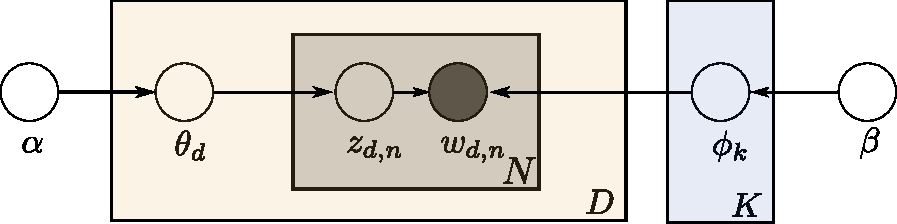
\includegraphics[scale=1.0]{./images/lda/lda.pdf}
\end{figure}
\begin{itemize}
	\item $\theta_d\sim Dir(\alpha)$: For each document, draw topic distribution. 
		\begin{itemize}
			\item $\alpha$: Dirichlet parameter
		\end{itemize}
	\item $z_{d,n}\sim Mult(\theta_d)$: per-word topic assignment. The $n$-th word of document $d$ is from which topic?
	\item $w_{d,n}\sim Mult(\phi_{z_{d,n}},n)$: observed word. The $n$-th word in a document $d$ is from a certain topic ($z_{d,n}$) distribution $\phi_{z_{d,n}}$.
	\item $\phi_k\sim Dir(\beta), i=\{1,\dots,K\}$: topics.
		\begin{itemize}
			\item $\beta$: topic hyperparameter (Dirichlet parameter).
		\end{itemize}
\end{itemize}
We can immediately notice that the LDA's modeling approach is quite far from the way we write texts. However, LDA works quite well. 

The document generation process can be modelled as follows:
\begin{align*}
	p(\phi_{1:K}, \theta_{1:D}, z_{1:D}, w_{1:D}) = \prod_{i=1}^K p(\phi_i|\beta)\prod_{d=1}^D p(\theta_d|\alpha)\Bigg(\prod_{n=1}^N p(w_{d,n}|\phi_{1:K},z_{d,n})p(z_{d,n}|\theta_d)\Bigg).
\end{align*}

\subsection{LDA Inference}
The posterior of the latent variables given the document is
\begin{align*}
	p(\phi, \theta, \mathbf{z}|\mathbf{w}) = \frac{p(\phi, \theta, \mathbf{z},\mathbf{w})}{\int_{\phi}\int_{\theta}\sum_{\mathbf{z}}p(\phi, \theta, \mathbf{z},\mathbf{w})}
\end{align*}
Computing the posterior is intractable:
\begin{itemize}
	\item The denominator is intractable
	\item We cannot compute the denominator, the marginal p(w).
	\item We are going to use collapsed Gibbs sampling. 
\end{itemize}

We want to estimate the topic distribution $\mathbf{z}$. 

\subsection{Dirichlet Distribution}
The Dirichlet Distribution can be considered as a extension of the \textit{beta distribution}. 
\begin{align}
	p(P=\{p_i\}|\alpha_i) = \frac{\Gamma(\sum_i\alpha_i)}{\prod_i\Gamma(\alpha_i)}\prod_ip_i^{\alpha_i-1}
	\label{eq:dirichlet_dist}
\end{align}
\begin{itemize}
	\item $\sum_ip_i = 1$
	\item The posterior distribution of Dirichlet distribution is also Dirichlet distribution. 
\end{itemize}
